\documentclass[12pt]{article}
\usepackage{preamble}
\usepackage{perltex}

\pagestyle{fancy}

\begin{document}
    \clearpage


    \section{X. Программа экзамена в 2023/2024}


    \begin{center}
        \textbf{5. Теория графов.}
    \end{center}


    \begin{enumerate}
        \item \textbf{Ориентированные и неориентированные графы} (\textit{Directed and undirected graphs})

        Граф - множество вершин $V$ и множество ребер $E$ (в общем случае), соединяющие какие-либо две вершины: $G(V, E)$

        По виду ребер различают:

        \smallvspace

        \begin{minipage}{0.45\textwidth}
            \begin{center}
                неориентированный граф

                \begin{tikzpicture}
                    \node[circle, draw=black!60, thick, minimum size=0.5cm] (v1) {$v_1$};
                    \node[circle, draw=black!60, thick, minimum size=0.5cm, above right=1cm and 1cm of v1] (v2) {$v_2$};
                    \node[circle, draw=black!60, thick, minimum size=0.5cm, below right=1cm and 1cm of v2] (v3) {$v_3$};
                    \node[circle, draw=black!60, thick, minimum size=0.5cm, below right=1cm and 1cm of v1] (v4) {$v_4$};
                    \node[circle, draw=black!60, thick, minimum size=0.5cm, right=1cm of v3] (v5) {$v_5$};
                    \path[-, ultra thick]
                    (v1) edge [] node {} (v2)
                    (v1) edge [] node {} (v3)
                    (v2) edge [] node {} (v3)
                    (v3) edge [] node {} (v4)
                    (v3) edge [] node {} (v5)
                    ;
                \end{tikzpicture}

                - ребра не имеют направлений
            \end{center}


        \end{minipage}%
        \hfill
        \begin{minipage}{0.45\textwidth}

            \begin{center}
                ориентированный граф

                \begin{tikzpicture}
                    \node[circle, draw=black!60, thick, minimum size=0.5cm] (v1) {$v_1$};
                    \node[circle, draw=black!60, thick, minimum size=0.5cm, above right=1cm and 1cm of v1] (v2) {$v_2$};
                    \node[circle, draw=black!60, thick, minimum size=0.5cm, below right=1cm and 1cm of v2] (v3) {$v_3$};
                    \node[circle, draw=black!60, thick, minimum size=0.5cm, below right=1cm and 1cm of v1] (v4) {$v_4$};
                    \node[circle, draw=black!60, thick, minimum size=0.5cm, right=1cm of v3] (v5) {$v_5$};
                    \path[->, ultra thick]
                    (v1) edge [] node {} (v2)
                    (v3) edge [] node {} (v1)
                    (v2) edge [] node {} (v3)
                    (v3) edge [] node {} (v2)
                    (v3) edge [] node {} (v4)
                    (v3) edge [] node {} (v5)
                    ;
                \end{tikzpicture}

                - ребра имеют направления

            \end{center}
        \end{minipage}

        \smallvspace


        \item \textbf{Простые графы и псевдографы} (\textit{Simple graphs and pseudographs})

        \smallvspace

        \begin{minipage}{\linewidth}
            \begin{wrapfigure}{r}{0pt}
                \begin{tikzpicture}
                    \node[circle, draw=black!60, thick, minimum size=0.5cm] (v1) {$v_1$};
                    \node[below=0.3cm of v1] (v2) {\small Петля};
                    \draw
                    (v1) edge [loop above] node {} (v1)
                    ;
                \end{tikzpicture}
            \end{wrapfigure}

            Простой граф $G(V, E)$ - граф, в котором
            \begin{itemize}
                \item $V \neq \emptyset$ - граф не пустой
                \item $E \subseteq V \times V$ - ребра представлены как множество пар вершин
                \item $\forall v \in V \ \Pair{v, v} \notin E$ - граф не содержит петлей - ребер, соединяющих одну вершину с собой же

            \end{itemize}

            Псевдограф $G(V, E)$ - простой граф, в котором разрешены петли

        \end{minipage}

        \smallvspace

        \item \textbf{Мультиребра и мультиграфы} (\textit{Multiedges and multigraphs})

        \begin{minipage}{\linewidth}
            \begin{wrapfigure}{r}{0pt}
                \begin{tikzpicture}
                    \node[circle, draw=black!60, thick] (v1) {};
                    \node[circle, draw=black!60, thick, above right=0.4cm and 0.4cm of v1] (v2) {};
                    \node[circle, draw=black!60, thick, below right=0.4cm and 0.4cm of v2] (v3) {};
                    \node[circle, draw=black!60, thick, below right=0.4cm and 0.4cm of v1] (v4) {};
                    \node[circle, draw=black!60, thick, right=0.4cm of v3] (v5) {};
                    \path[-]
                    (v1) edge [] node {} (v2)
                    (v3) edge [] node {} (v1)
                    (v3) edge [] node {} (v2)
                    (v3) edge [bend right] node {} (v2)
                    (v1) edge [bend right] node {} (v4)
                    (v1) edge [bend left] node {} (v4)
                    (v3) edge [] node {} (v5)
                    (v3) edge [bend right] node {} (v5)
                    (v3) edge [bend left] node {} (v5)
                    ;
                \end{tikzpicture}
            \end{wrapfigure}

            \smallvspace


            Мультиребра - ребра, соединяющие одну и ту же пару вершин больше одного раза

            Мультиграфы - графы, содержащие мультиребра. В этом случае $E$ - мультимножество
        \end{minipage}

        \begin{minipage}{\linewidth}
            \begin{wrapfigure}{R}{-10pt}
                \begin{tikzpicture}
                    \node[circle, draw=black!60, thick] (v1) {};
                    \node[circle, draw=black!60, thick, right=0.4cm of v1] (v2) {};
                    \node[circle, draw=black!60, thick, right=0.4cm of v2] (v3) {};
                    \node[circle, draw=black!60, thick, right=0.4cm of v3] (v4) {};
                    \node[circle, draw=black!60, thick, below right=0.4cm and 0.2cm of v2] (v5) {};
                    \draw[rounded corners] ([xshift=-0.2cm,yshift=-0.3cm]v1.west) rectangle ([xshift=0.2cm,yshift=0.3cm]v4.east) {};
                    \node[above right=0.2cm and -0.15cm of v1] (vcc) {гиперребро};
                    \path[-]
                    (v3) edge [bend left] node {} (v5)
                    (v1) edge [bend right] node {} (v5)
                    ;
                \end{tikzpicture}
            \end{wrapfigure}

            \smallvspace

            \item \textbf{Гиперграфы} (\textit{Hypergraphs})

            Гиперребро - ребро, соединяющее несколько вершин

            Гиперграф - граф, содержащий гиперребро
        \end{minipage}

        \bigvspace

        \item \textbf{Нуль-граф, пустой граф и синглтон} (\textit{Null, empty, singleton graphs})

        Нуль-граф - граф, не содержащий вершин (и ребер)

        Пустой граф - граф, не содержащий ребер

        Синглтон - граф, содержащий из одной вершины

        \smallvspace

        \item \textbf{Полный граф} (\textit{Complete graph})

        Полный граф $K_n$ - простой граф из $n$ вершин, в которой все вершин соединены друг с другом

        \begin{center}
            \begin{tikzpicture}
                \node[circle, draw=black!60, thick] (v1) {};
                \node[circle, draw=black!60, thick, right=0.5cm of v1] (v2) {};
                \node[below right=1.2cm and -0.25cm of v1] (vcc) {$n = 2$};
                \path[-]
                (v1) edge [] node {} (v2)
                ;
                \node[circle, draw=black!60, thick, right=2.5cm of v2] (p1) {};
                \node[circle, draw=black!60, thick, below right=0.5cm and 0.25cm of p1] (p2) {};
                \node[circle, draw=black!60, thick, below left=0.5cm and 0.25cm of p1] (p3) {};
                \node[below right=0.4cm and -0.25cm of p3] (pcc) {$n = 3$};
                \path[-]
                (p1) edge [] node {} (p2)
                (p1) edge [] node {} (p3)
                (p3) edge [] node {} (p2)
                ;
                \node[circle, draw=black!60, thick, right=2.5cm of p1] (q1) {};
                \node[circle, draw=black!60, thick, right=0.5cm of q1] (q2) {};
                \node[circle, draw=black!60, thick, below=0.5cm of q1] (q3) {};
                \node[circle, draw=black!60, thick, right=0.5cm of q3] (q4) {};
                \node[below right=0.3cm and -0.25cm of q3] (qcc) {$n = 4$};
                \path[-]
                (q1) edge [] node {} (q2)
                (q1) edge [] node {} (q3)
                (q1) edge [] node {} (q4)
                (q2) edge [] node {} (q3)
                (q2) edge [] node {} (q4)
                (q3) edge [] node {} (q4)
                ;
            \end{tikzpicture}
        \end{center}

        \item \textbf{Взвешенный граф} (\textit{Weighted graph})

        Взвешенный граф - граф, в котором ребра (и/или вершины) имеют числовой вес.
        Иначе говоря, определена функция $w \ : \ E \to \Real$

        \item \textbf{Планарный граф} (\textit{Planar graphs})

        Планарный граф - граф, который можно изобразить на плоскости без пересечений рёбер

        По теореме Понтрягина-Куратовского граф планарен \textit{тогда и только тогда, когда}
        он не содержит подграфов, гомеоморфных полному графу из пяти вершин K\textsubscript{5} или графу «домики и колодцы» K\textsubscript{3,3}


        \item \textbf{Подграф} (\textit{Subgraph})

        Подграф графа $G(V, E)$ - граф $G^\prime(V^\prime, E^\prime)$
        такой, что $V^\prime \subseteq V, E^\prime \subseteq E$

        \item \textbf{Остовный подграф} (\textit{Spanning subgraph})

        Остовный подграф графа $G(V, E)$ - такой подграф $G^\prime(V, E^\prime)$, содержащий все вершины исходного


        \item \textbf{Порожденный подграф} (\textit{Induced subgraph})

        Порожденный подграф $G[S]$ графа $G(V, E)$ - подграф $G^\prime(S, E^\prime)$, который содержит все ребра, соединяющие вершины из $S$ в исходном графе

        \item \textbf{Отношение смежности} (\textit{Adjacency relation})

        Отношение смежности - отношение $A$ между вершинами, соединенными ребром: $A = \Set{\Pair{u, v} \ | \ \Pair{u, v} \in E}$

        \item \textbf{Матрица смежности} (\textit{Adjacency matrix})

        Матрица смежности - матрица $A_{V\timesV}$, выражающее отношение смежности

        % TODO picture

        \item \textbf{Отношение инцидентности} (\textit{Incidence relation})

        Отношение инцидентности - отношение $B$ между вершиной и соединяющей ее ребром: $B = \Set{\Pair{u, e} \ | \ u \in V \land e \in E \land \exists v \in V \ | \ (\Pair{u, v} \in E \lor \Pair{v, u} \in E)}$

        \item \textbf{Матрица инцидентности} (\textit{Incidence matrix})

        Матрица инцидентности - матрица $A_{V\timesV}$, выражающее отношение инцидентности

        % TODO picture

        \item \textbf{Степень вершины} (\textit{Vertex degree})

        Степень $\deg(v)$ вершины $v$ - количество и ребер из этой вершины (петли считаются дважды)

        Назовем $\delta(G)$ - минимальная степень вершины в графе, $\Delta(G)$ - максимальная степень вершины в графе

        \item \textbf{Регулярный граф} (\textit{Regular graph})

        $r$-регулярный граф - граф, все степени вершин которого равны $r$ - $\forall v \in V \ \deg(v) = r$

        \item \textbf{Лемма о рукопожатиях} (\textit{Handshaking lemma})

        $\sum_{v \in V} \deg(v) = 2|E|$ - сумма степеней всех вершин равна удвоенному количеству ребер

        \item \textbf{Изоморфизм графов} (\textit{Graph isomorphism})

        Графы $G(V, E)$ и $H(U, F)$ называются изоморфными, если существует биекция $f \ | \ V \to U$ такая, что
        если вершины $v$ и $u$ графа $G$ смежны, то и вершины $f(v)$ и $f(u)$ графа $H$ тоже смежны

        \begin{minipage}{\linewidth}
            \begin{wrapfigure}{r}{0.4\linewidth}
                \begin{center}
                    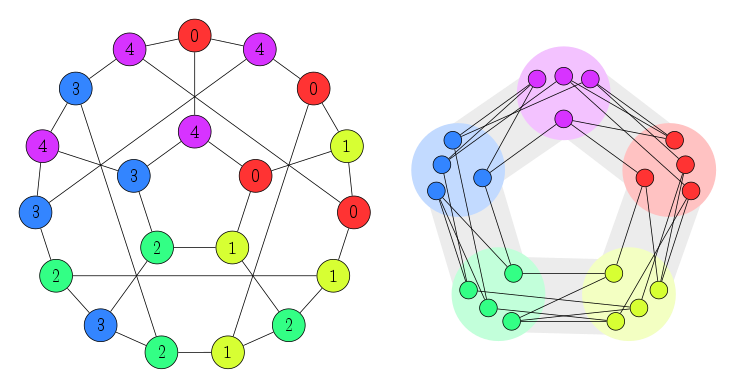
\includegraphics[width=\linewidth]{dismath/images/dismath_exam_list_graph_homomorphism}

                    Гомоморфизм

                    \smallvspace

                    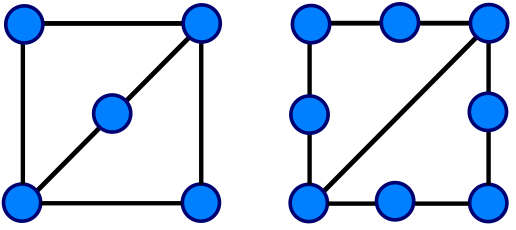
\includegraphics[width=\linewidth]{dismath/images/dismath_exam_list_graph_homeomorphism}

                    Гомеоморфизм
                \end{center}
            \end{wrapfigure}

            \smallvspace

            \item \textbf{Гомоморфизм графов} (\textit{Graph homomorphism})

            Гомоморфизм графов - отображение вершин графа $G$ в вершины графа $H$ такое,
            что смежные вершины графа $G$ отображаются в смежные вершины графа $H$


            \item \textbf{Гомеоморфизм графов} (\textit{Graph homeomorphism})

            Деление (Subdivision) ребра $\Pair{u, v}$ - операция, добавляющее верщину $w$, ребра $\Pair{u, w}$ и $\Pair{w, v}$ и удаляющее ребро $\Pair{u, v}$

            Исключение (Smoothing) вершины $w$ (степени 2) - операция, обратная делению - исключение вершины $w$ и ребер $\Pair{u, w}$ и $\Pair{w, v}$ и добавление ребра $\Pair{u, v}$

            Графы $G$ и $H$ гомеоморфны, если граф $H$ можно получить в результате деления или исключения графа $G$

        \end{minipage}

        \smallvspace

        \item \textbf{Пути и циклы} (\textit{Walks, paths, trails, cycles})

        Путь (Walk) - последовательность из вершин и ребер, соединяющих соседние вершины: $l = (v_0, e_0, v_1, e_1, \dots, e_{n - 1}, v_n)$

        Цепь (Trail) - путь (walk), все ребра которого различны

        Простая цепь (Path) - путь (walk), все вершины (и соответственно ребра) которого различны

        Замкнутый путь (Closed walk) - путь (walk), начальная вершина которого является конечной

        Контур (Circuit) - цепь (trail), являющаяся замкнутым

        Цикл (Cycle) - простая цепь (path), являющаяся замкнутым

        (*терминология из Википедии)


        \item \textbf{Эйлеровы путь, цикл, граф} (\textit{Eulerian path, cycle, graph})

        Эйлеров путь - путь, содержащий все ребра графа

        Эйлеров цикл - замкнутый путь, содержащий все ребра графа

        Граф называют эйлеровым, если в нем есть эйлеров цикл. Граф называют полуэйлеровым, если в ней есть эйлеров путь.

        \item \textbf{Теорема Эйлера для графов} (\textit{Euler's theorem for graphs})

        Граф эйлеров, если все степени вершин четные, а ребра принадлежат одной компоненте связности

        Граф полуэйлеров, если ровно 2 вершины имеют нечетную степень, а ребра принадлежат одной компоненте связности

        \item \textbf{Гамильтоновы путь, цикл, граф} (\textit{Hamiltonian path, cycle, graph})

        Гамильтонов путь - путь, содержащий все вершины графа

        Гамильтонов цикл - замкнутый путь, содержащий все вершины графа

        Граф называют гамильтоновым, если в нем есть гамильтонов цикл. Граф называют полугамильтоновым, если в ней есть гамильтонов путь.

        \item \textbf{Теорема Оре} (\textit{Ore’s theorem})

        Теорема Оре - достаточное условие существования гамильтонова цикла: если в графе $G(V, E)$ для любых $u, v \in V$ $\deg u + \deg v \geq |V|$, то граф $G$ гамильтонов

        \item \textbf{Теорема Дирака} (\textit{Dirac’s theorem})

        Теорема Дирака - достаточное условие существования гамильтонова цикла: если в графе $G(V, E)$ для любой $u \in V$ $\deg u \geq \frac{|V|}{2}$, то граф $G$ гамильтонов


        \item \textbf{Эксцентриситет вершины} (\textit{Eccentricity of a vertex})

        Расстояние $\text{dist}(u, v)$ - длина (количество ребер) кратчайшего пути между $u$ и $v$

        Эксцентриситет $\varepsilon(v)$ - наибольшая длина кратчайшего пути от этой вершины до другой в этом графе: $\varepsilon(v) = \max_{u \in V} \text{dist}(v, u)$

        \item \textbf{Радиус и диаметр графа} (\textit{Radius and diameter of a graph})

        Радиус графа $\text{rad}(G)$ - наименьший эксцентриситет вершины из графа: $\text{rad}(G) = \min_{v \in V} \varepsilon(v)$

        Диаметр графа $\text{diam}(G)$ - наибольший эксцентриситет вершины из графа: $\text{diam}(G) = \max_{v \in V} \varepsilon(v)$

        \item \textbf{Центр графа} (\textit{Center of a graph})

        Центр графа - вершина (вершины), эксцентриситет которой равен радиусу графа: $\text{center}(G) = \Set{v \in V \ | \ \varepsilon(v) = \text{rad}(G)}$

        \item \textbf{Центроид дерева} (\textit{Centroid of a tree})

        Центроид дерева - вершина (или 2 вершины), удаление которой приведет к распаду на поддеревья, каждое из которое имеет не больше $\frac{|V|}{2}$ вершин

        Очевидно, что только деревья, состоящие из четного количества вершин, могут иметь 2 центроида

        % TODO picture

        \item \textbf{Клика} (\textit{Clique})

        Клика графа - порожденный подграф, который является полный графом. $1$-клика - вершина, $2$-клика - 2 вершины и ребро, $3$-клика - треугольник, $n$-клика - граф $K_n$

        \item \textbf{Независимое (стабильное множество)} (\textit{Independent set})

        Независимое (стабильное) множество - множество вершин, каждая из которых не соединена ребром с другой вершиной из множества

        \item \textbf{Паросочетание} (\textit{Matching})

        Паросочетание (независимое множество ребер) - множество ребер, каждые из которые не соединяют одну и ту же вершину

        \item \textbf{Идеальное паросочетание} (\textit{Perfect matching})

        Идеальное паросочетание - паросочетание, ребра которого инцидентны ко всем вершинам графа (то есть паросочетание, являющееся реберным покрытием)

        \item \textbf{Вершинное покрытие} (\textit{Vertex cover})

        Вершинное покрытие - множество вершин, к которым инцидентны все ребра графа

        \item \textbf{Реберное покрытие} (\textit{Edge cover})

        Реберное покрытие - множество ребер, которые инцидентны ко всем вершинам

        \item \textbf{Дерево} (\textit{Tree})

        Дерево - связный ацикличный граф

        \item \textbf{Лес} (\textit{Forest})

        Лес - несвязный граф, каждая компонента которого не имеет циклов (граф, состоящий из деревьев)

        \item \textbf{Минимальное остовное дерево} (\textit{Minimum spanning tree})

        Минимальное остовное дерево взвешенного графа $G(V, E, w)$ - дерево $T(V, E^\prime)$, сумма весов ребер которого имеет наименьшее значение

        \item \textbf{Код Прюфера} (\textit{Prüfer code})

        Код Прюфера - алгоритм кодировки маркированного дерева размера $n$ в последовательность чисел

        \textbf{Кодировка}:

        1. Делаем биекцию между названиями вершин и числа из диапазона $[1;n]$ (если необходимо)

        2. Берем лист с наименьшим значением, удаляем его, записываем в последовательность номер его родителя

        3. Повторяем 2. до тех пор, пока не останется 2 вершины - их кодировка тривиальна и не нуждается в хранении

        \textbf{Декодировка}:

        1. Создаем $n$ вершин, и множество вершин $W$, которых нет в последовательности

        2. Читаем номер вершины из последовательности

        3. Соединяем эту вершину с вершиной из $W$ с минимальным номером, удалив ее

        4. Добавляем вершину из последовательности в $W$

        5. Повторяем 2.-4.

        6. Соединяем 2 оставшиеся вершины из $W$


        \item \textbf{Двудольный граф} (\textit{Bipartite graph})

        Двудольный граф $K_{n,m}$ - граф, вершины которого можно разбить на две части размеров $n$ и $m$ таким образом, что вершины из одной части не смежны друг с другом

        \item \textbf{Теорема баланса регулярных двудольных графов} (\textit{Theorem on the balance of regular bipartite graphs})

        Если двудольный граф $K_{n,m}$ регулярный, то $n = m$

        $\Box$ Граф регулярный $\Longrightarrow \forall v \in V \ \deg v = r \in \Natural \Longrightarrow $ левая доля имеет $nr$ исходящих ребер, а правая доля имеет $mr$ входящих ребер, но так как вершины в долях не соединены ребрами, $nr = mr$ $\Box$

        \item \textbf{Теорема существования идеального паросочетания регулярного двудольного графа} (\textit{Theorem on the existence of a perfect matching in a regular bipartite graph})

        Теорема: у любого $r$-регулярного двудольного графа ($r > 0$) существует идеальное паросочетание

        $\Box$

        Пусть $G(V, E)$ - граф, вершины разбиваются на две доли $X \xor Y = V$

        Пусть $N(A) = \Set{y \in Y \ | \ \exists x \in X \ \Pair{x, y} \in E}$ - соседи (смежные вершины) вершин из множества $A \subseteq X$

        Докажем от противного: пусть идеального паросочетания не существует, тогда по теореме Холла $\exists S \subset X \ | \ |S| > |N(S)|$,
        но тогда кол-во ребер, выходящих из $S$, равно $r|S|$, но кол-во ребер, выходящих из $N(S)$, равно $r|N(S)|$

        Из этого $r|S| > r|N(S)|$, что невозможно, так как $N(S)$ - соседи $S$ - противоречие

        $\Box$


        \item \textbf{Теорема Холла} (\textit{Hall's theorem (on the existence of an X-perfect matching in a bipartite graph)})

        Пусть $G(V, E)$ - граф, вершины разбиваются на две доли $X \xor Y = V$

        Тогда в графе $G(V, E)$ существует $X$-идеальное паросочетание (паросочетание, покрывающее все вершины $X$) тогда и только тогда,
        когда для любого $A \subset X \ |A| \leq |N(A)|$

        $\Box$ Если существует такое $A$, что $|A| > |N(A)|$, то какой-либо вершине из $A$ не найдется противоположная вершина из $N(A)$ и $X$-идеального паросочетания не выйдет $\Box$


        \item \textbf{Связность в неориентированных графах} (\textit{Connectivity in undirected graphs})

        Компонента связность графа - максимальный подграф, в котором от каждой вершины до любой другой существует путь

        Граф считается связным, если он представляет собой одну компоненту связности

        \item \textbf{Сильная и слабая связность в ориентированных графах} (\textit{Strong and weak connectivity in directed graphs})

        Компонента сильной связности - максимальный подграф, в котором для любых вершин $u, v$ существует пути $u \rightsquigarrow v$ и $v \rightsquigarrow u$

        Компонента слабой связности - максимальный подграф, который является компонентой связности в неориентированном графе, полученном при удалении ориентации ребер у исходного

        % TODO picture

        \item \textbf{Конденсация ориентированного графа} (\textit{Condensation of a directed graph})

        Конденсация графа - сжатие сильно связных компонент графа до вершин с целью получения упрощенного и ациклического графа

        \item \textbf{Вершинная связность} (\textit{Vertex connectivity})

        Вершинная связность $\kappa(G)$ графа $G$ - минимальное число вершин, которое нужно удалить в графе, чтобы он стал несвязным или синглтоном

        \item \textbf{Реберная связность} (\textit{Edge connectivity})

        Реберная связность $\lambda(G)$ графа $G$ - минимальное число ребер, которое нужно удалить в графе, чтобы он стал несвязным

        \item \textbf{Теорема Уитни} (\textit{Whitney's theorem})

        Для любого графа $\kappa(G) \leq \lambda(G) \leq \delta(G)$

        $\Box$

        Допустим, что $\kappa(G) > \lambda(G)$, тогда после удаления $\lambda(G)$ ребер будет $k \leq \lambda(G)$ вершин со одной стороны и $m \leq \lambda(G)$ с другой.
        Но мы их тоже можем удалить, и граф распадется, значит $\lambda < \kappa(G) = \min (k, m) \leq \lambda(G)$ - противоречие

        Допустим, что $\lambda(G) > \delta(G)$, тогда мы можем найти в графе вершину с наименьшей степенью $\delta(G)$,
        при удалении $\delta(G)$ ребер граф распадется, значит $\lambda(G) = \delta(G)$ - противоречие

        $\Box$


        \item \textbf{$k$-связный граф} (\textit{k-connected graph})

        $k$-вершинно-связный граф - граф, остающийся связным после удаления $k$ вершин ($\kappa(G) \geq k$).

        НО: синглтон имеет $\kappa(G) = 0$, он не $1$-вершинно-связный, при этом он связный; $K_2$ имеет $\kappa(G) = 1$,
        поэтому он не $2$-вершинно-связный, но $K_2$ может быть блоком

        $k$-реберно-связный граф - граф, остающийся связным после удаления $k$ ребер ($\lambda(G) \geq k$)

        НО: у синглтона $\lambda(G) = 0$, он не $1$-реберно-связный, при этом синглтон - компонента реберной двусвязности

        \item \textbf{Теорема Менгера} (\textit{Menger's theorem})

        Теорема (Менгера о реберной двойственности в ориентированном графе):

        Между вершинами $u$ и $v$ существует $L$ реберно непересекающихся путей тогда и только тогда,
        когда после удаления любых $(L - 1)$ ребер существует путь из $u$ в $v$.

        Теорема (Менгера о вершинной двойственности в ориентированном графе):

        Между вершинами $u$ и $v$ существует $L$ вершинно непересекающихся путей тогда и только тогда,
        когда после удаления любых $(L - 1)$ вершин существует путь из $u$ в $v$.

        \href{https://neerc.ifmo.ru/wiki/index.php?title=%D0%A2%D0%B5%D0%BE%D1%80%D0%B5%D0%BC%D0%B0_%D0%9C%D0%B5%D0%BD%D0%B3%D0%B5%D1%80%D0%B0#.D0.A2.D0.B5.D0.BE.D1.80.D0.B5.D0.BC.D0.B0}{Доказательства}


        \item \textbf{Двусвязность} (\textit{Biconnectivity})

        Двусвязность (вершинная) определяется как отношение эквивалентности 2 ребер, между концами которых существуют 2 вершинно-различных пути  % a little strange

        Компонента (вершинной) двусвязности (также блок) - подграф, который включает все двусвязные ребра (класс эквивалентности двусвязности).

        Реберная двусвязность определяется как отношение эквивалентности 2 вершины, между которыми существуют 2 реберно-различных пути

        Компонента реберной двусвязности - подграф, который включает все двусвязные вершины (класс эквивалентности двусвязности).

        \item \textbf{Точка сочленения} (\textit{Articulation point})

        Точка сочленения - вершина, принадлежащая нескольким компонентам (вершинной) двусвязности

        \item \textbf{Мост} (\textit{Bridge})

        Мост - ребро, соединяющее две компоненты реберной двусвязности

        \item \textbf{Блок} (\textit{Blocks})

        Блок - компонента вершинной двусвязности

        \item \textbf{Дерево блоков и точек сочленений} (\textit{Block-cut tree})

        Дерево блоков и точек сочленений графа - дерево, в котором каждая вершина представляет собой либо точку сочленения, либо блок,
        при этом вершина точки сочленения соединена только с вершиной блока и наоборот

        % TODO bc-tree picture

    \end{enumerate}

    \begin{center}
        \textbf{6. Теория автоматов.}
    \end{center}


    \begin{enumerate}
        \item \textbf{} (\textit{Deterministic Finite Automaton (DFA)})

        \item \textbf{} (\textit{Non-deterministic Finite Automaton (NFA)})

        \item \textbf{} (\textit{Formal languages})

        \item \textbf{} (\textit{Operations on formal languages (concat, union, Kleene closure)})

        \item \textbf{} (\textit{Regular languages})

        \item \textbf{} (\textit{Regular expression})

        \item \textbf{} (\textit{Kleene's theorem})

        \item \textbf{} (\textit{Powerset construction (DFA from NFA)})

        \item \textbf{} (\textit{$\varepsilon$-NFA})

        \item \textbf{} (\textit{NFA construction from $\varepsilon$-NFA})

        \item \textbf{} (\textit{Thompson’s construction ($\varepsilon$-NFA from regular expression)})

        \item \textbf{} (\textit{Kleene’s algorithm})

        \item \textbf{} (\textit{Pumping lemma for regular languages})

        \item \textbf{} (\textit{Closure properties of regular languages})

        \item \textbf{} (\textit{Mealy machine})

        \item \textbf{} (\textit{Moore machine})

        \item \textbf{} (\textit{Emptiness of finite automaton language})

        \item \textbf{} (\textit{Finiteness of finite automaton language})

        \item \textbf{} (\textit{Equivalence of finite automata})

        \item \textbf{} (\textit{Myhill-Nerode theorem})

    \end{enumerate}


    \begin{center}
        \textbf{7. Комбинаторика.}
    \end{center}


    \begin{enumerate}
        \item \textbf{} (\textit{Ordered arrangements})

        \item \textbf{} (\textit{Permutations})

        \item \textbf{} (\textit{k-permutations})

        \item \textbf{} (\textit{Cyclic permutations})

        \item \textbf{} (\textit{Unordered arrangements})

        \item \textbf{} (\textit{k-combinations})

        \item \textbf{} (\textit{Multisets})

        \item \textbf{} (\textit{Permutations of multisets})

        \item \textbf{} (\textit{Combinations of infinite multisets})

        \item \textbf{} (\textit{Compositions})

        \item \textbf{} (\textit{Set partitions})

        \item \textbf{} (\textit{Stirling numbers of the second kind})

        \item \textbf{} (\textit{Integer partitions})

        \item \textbf{} (\textit{Principle of Inclusion-Exclusion})

    \end{enumerate}

    \begin{center}
        \textbf{8. Рекуррентности и производящие функции.}
    \end{center}


    \begin{enumerate}
        \item \textbf{} (\textit{Recurrence relations})

        \item \textbf{} (\textit{Solving recurrence relations using characteristic equations})

        \item \textbf{} (\textit{Generating functions})

        \item \textbf{} (\textit{Power series})

        \item \textbf{} (\textit{Solving linear recurrences using generating functions})

        \item \textbf{} (\textit{Solving combinatorial problems using generating functions})

        \item \textbf{} (\textit{Operators and annihilators})

        \item \textbf{} (\textit{Solving linear recurrences using annihilators})

        \item \textbf{} (\textit{Catalan numbers})

        \item \textbf{} (\textit{Divide-and-Conquer algorithms analysis using recursion trees})

        \item \textbf{} (\textit{Master theorem})

        \item \textbf{} (\textit{Akra-Bazzi method})

    \end{enumerate}


\end{document}